\subsection{Domänenmodell}\label{l:domänenmodell}

\begin{center}
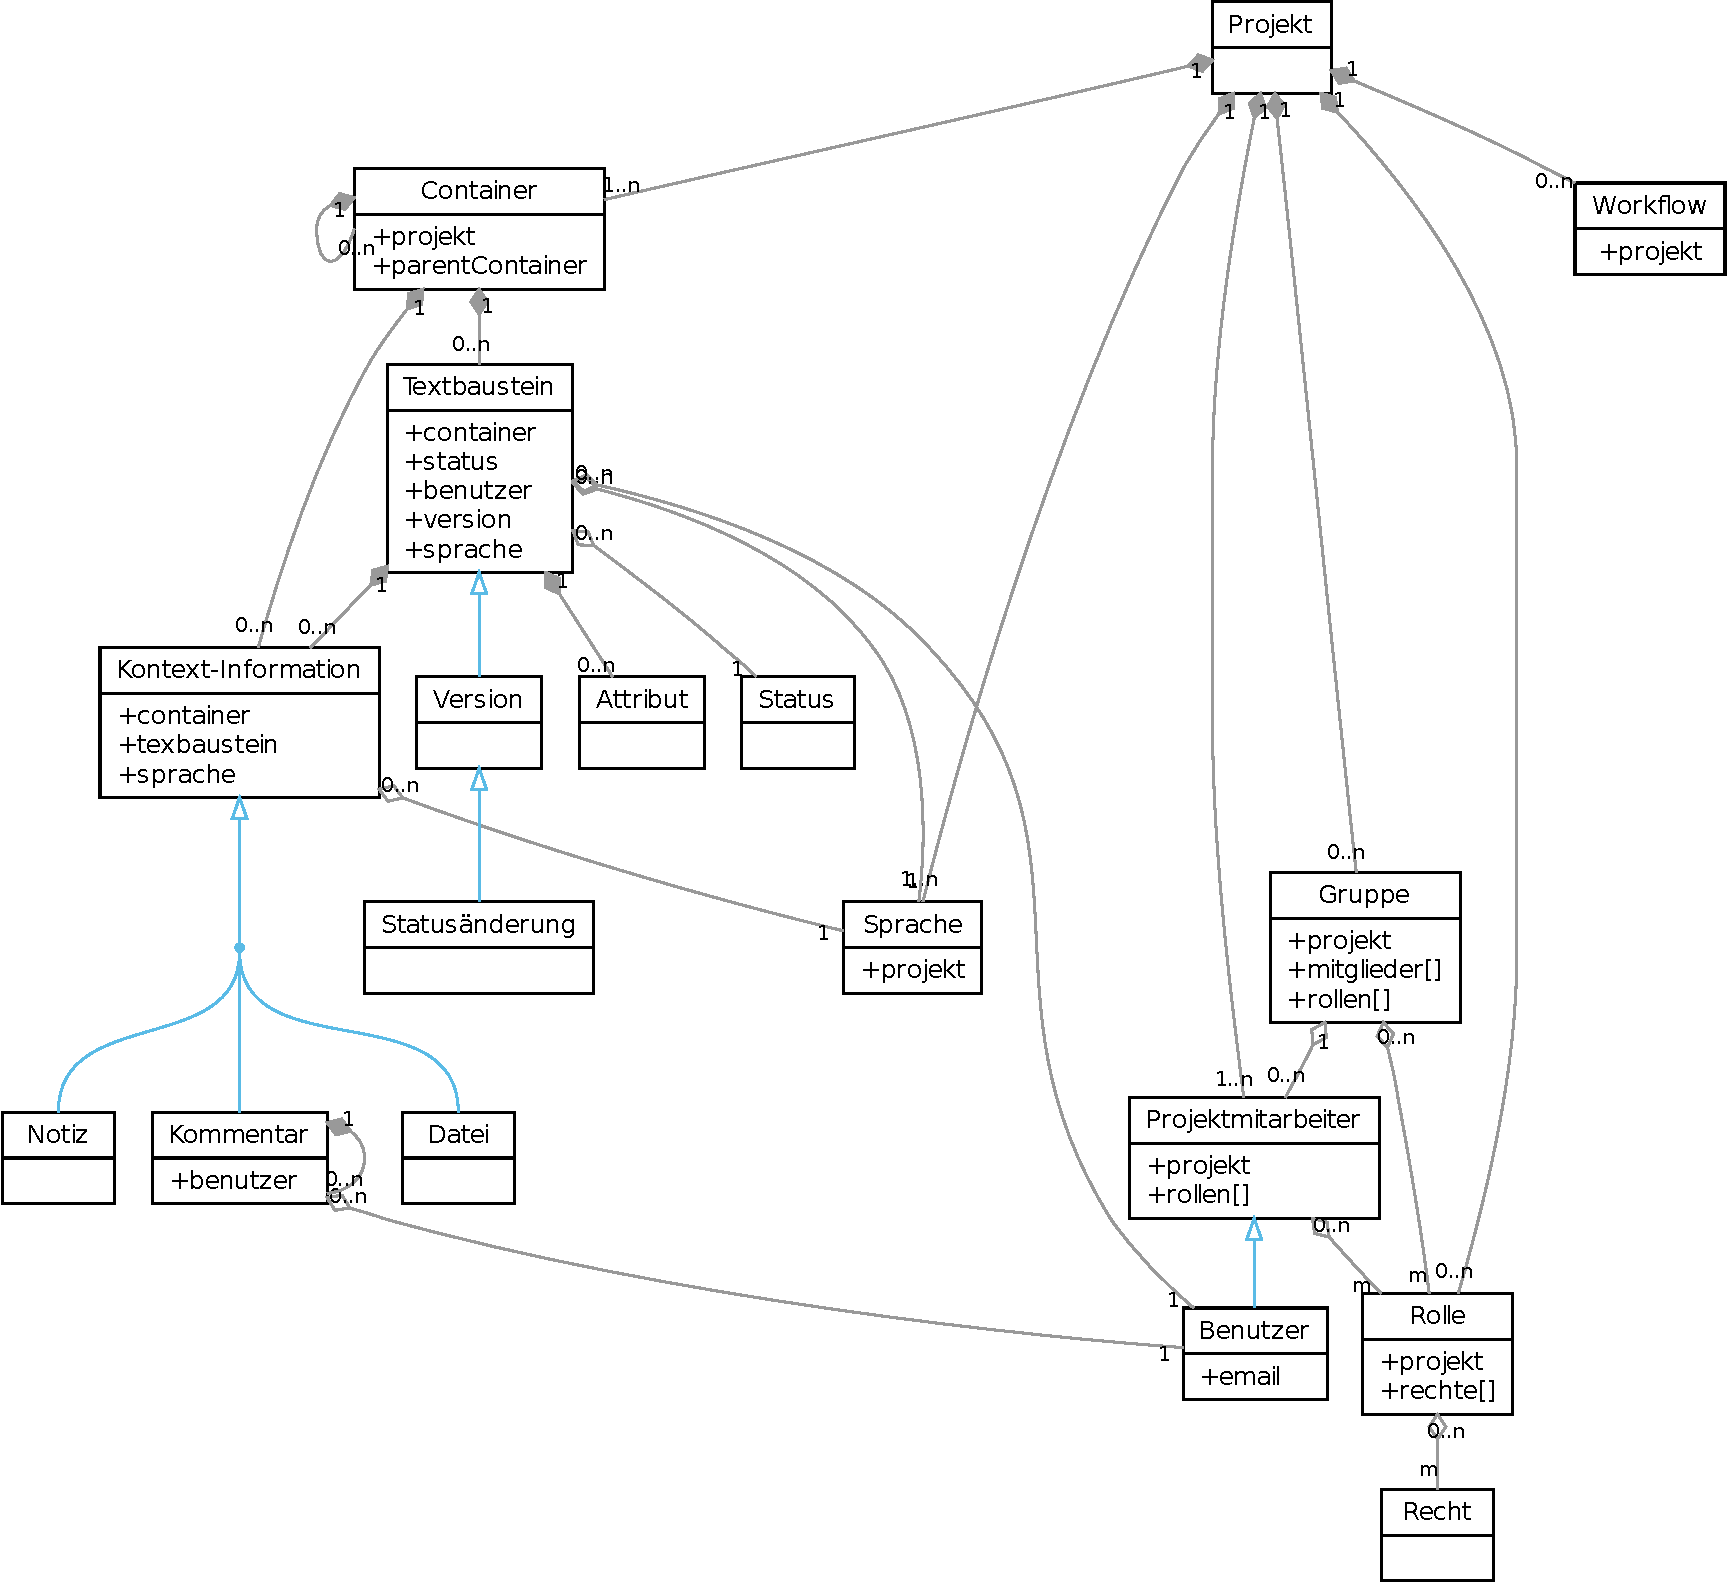
\includegraphics[width=\textwidth]{media/domain.pdf}
\captionof{figure}{Domänenmodell}\label{chart:domain}
\end{center}

Aus den vorangegangenen Überlegungen zur Anwendung und zum Workflow lässt sich ein Domänenmodell extrahieren, die einzelnen logischen Objekte innerhalb der Anwendung beschreibt, mit deren Hilfe alle Operationen abgebildet werden. Abbildung~\ref{chart:domain} zeigt das Modell in der Übersicht, dass die sich im Entwurf der Anwendung in deren Implementierung im Prototypen widerspiegelt.

\textsf{\textbf{Attribut}}\\Beschreibt die Attribute eines Textbausteins.

\textsf{\textbf{Benutzer}}\\Repräsentiert einen Benutzer des Systems

\textsf{\textbf{Container}}\\Containern dienen zur hierarchischen Organisation der Texte innerhalb des Projekts. Containern können weitere Container und Texte enthalten. Eine Container ohne übergeordneten Container befindet sich auf der obersten Ebene. Es kann mehrere Containern auf der obersten Ebene geben.

\textsf{\textbf{Gruppe}}\\Mitarbeiter können in Gruppen zusammengefasst werden. Dies erleichtert die Konfiguration des Workflows und der Rechte.

\textsf{\textbf{Kommentare}}\\Kommentare enthalten Hinweise und Fragen zu einzelnen Texten und Texbausteinen.

\textsf{\textbf{Kontext-Information}}\\Projektspezifische Kontext-Informationen lassen sich hinterlegen und Textbausteinen und Containern zuordnen.

\textsf{\textbf{Projekt}}\\Projekte bildet den Rahmen für alle Texte eines einzelnen Produktes.

\textsf{\textbf{Projektmitarbeiter}}\\Gestattet einem Benutzer die Mitarbeit an einem Projekt und legt dabei fest, welche Rechte dem Benutzer für das Projekt zustehen.

\textsf{\textbf{Recht}}\\Beschreibt ein Recht, eine Operation auf einem Objekt auszuführen.

\textsf{\textbf{Rolle}}\\Beschreibt die verschiedenen Rollen innerhalb der Anwendung. Die Rechte der Rollen sind durch die Zuordnung von Benutzern zu Projekten durch den Projektmitarbeiter immer an das jeweilige Projekt gebunden.

\textsf{\textbf{Sprache}}\\Die Texte jedes Projekts liegen in einer oder mehreren Sprachen vor.

\textsf{\textbf{Status}}\\Beschreibt die verschiedenen Zustände eines Textbausteins (vgl. Abschnitt \ref{l:konzept-workflow-status} · S.\pageref{l:konzept-workflow-status}).

\begin{enumerate}\itemsep -5pt
\item \texttt{Neu}, Textbaustein erzeugt
\item \texttt{Leer}, Textbaustein definiert
\item \texttt{Befüllt}, Textbaustein mit Inhalt befüllt
\item \texttt{Korrigiert}, Orthografie geprüft
\item \texttt{Geprüft}, Inhalt geprüft (Qualitätsicherung)
\item \texttt{Freigegeben}, durch Kunden freigegeben
\item \texttt{Veröffentlicht}, in Produkt übernommen
\end{enumerate}

\textsf{\textbf{Statusänderung}}\\Beschreibt eine Änderung eines Status durch einen Benutzer, z.B. durch Freigabe oder Überprüfung.

\textsf{\textbf{Textbaustein}}\\Beschreibt einen einzelnen Textbaustein.

\textsf{\textbf{Version}}\\Beschreibt eine Version des Inhalts eines Textbausteins.

\textsf{\textbf{Workflow}}\\Beschreibt einen projektspezifischen Workflow.
